% Gerado por scripts/gerar_artigo.py a partir dos JSONs em experimentos/*/resultados. Não editar à mão.
\newcommand{\EtrezeTarefa}{88,5}
\newcommand{\EtrezeInter}{6,7}
\newcommand{\EtrezeAlg}{2,8}
\newcommand{\EtrezeInit}{1,9}
\newcommand{\EtrezeArq}{0,2}
\newcommand{\EtrezeZG}{2,5}
\newcommand{\EtrezeExpK}{1,79}
\newcommand{\EtrezeRazaoLarga}{0,90}
\newcommand{\EtrezeExec}{72}
\newcommand{\EtrezeCens}{0}
\newcommand{\EtrezeHdoze}{8}
\newcommand{\EtrezeAlvoDois}{89,3}
\newcommand{\EtrezeRefDois}{99,1}
\newcommand{\EtrezeAlvoCinco}{75,8}
\newcommand{\EtrezeRefCinco}{89,8}
\newcommand{\EtrezeAlvoDez}{72,3}
\newcommand{\EtrezeRefDez}{87,8}
\newcommand{\EtrezeTabela}{%
\begin{table}[t]
\centering
\caption{E13: bits entregues até o alvo, $I$ (média geométrica de 3 sementes)}
\label{tab:e13}
\begin{tabular}{lllrrr}
\toprule
Arq. & Inic. & Alg. & $k=2$ & $k=5$ & $k=10$ \\
\midrule
prof. & padrão & Adam & 2.663 & 18.253 & 38.307 \\
prof. & padrão & SGDM & 3.804 & 37.218 & 67.621 \\
prof. & Xavier & Adam & 2.032 & 17.539 & 29.868 \\
prof. & Xavier & SGDM & 1.465 & 11.820 & 22.119 \\
larga & padrão & Adam & 1.016 & 10.336 & 23.465 \\
larga & padrão & SGDM & 2.547 & 33.139 & 84.583 \\
larga & Xavier & Adam & 2.225 & 11.065 & 24.477 \\
larga & Xavier & SGDM & 2.663 & 17.056 & 40.987 \\
\bottomrule
\end{tabular}
\end{table}}
\newcommand{\EtrezeFigura}{%
\begin{figure}[t]
\centering
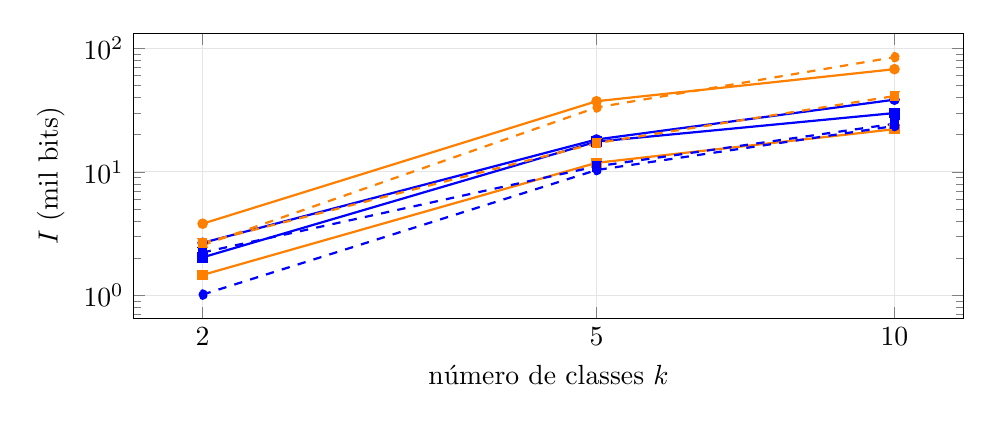
\begin{tikzpicture}
\begin{axis}[width=\columnwidth, height=5.2cm, xmode=log, ymode=log, log basis x=2, xtick={2,5,10}, xticklabels={2,5,10}, xlabel={número de classes $k$}, ylabel={$I$ (mil bits)}, grid=major, grid style={gray!20}, every axis plot/.append style={thick}]
\addplot[blue, solid, mark=*, mark size=1.5pt] coordinates {(2,2.663) (5,18.253) (10,38.307)};
\addplot[orange, solid, mark=*, mark size=1.5pt] coordinates {(2,3.804) (5,37.218) (10,67.621)};
\addplot[blue, solid, mark=square*, mark size=1.5pt] coordinates {(2,2.032) (5,17.539) (10,29.868)};
\addplot[orange, solid, mark=square*, mark size=1.5pt] coordinates {(2,1.465) (5,11.820) (10,22.119)};
\addplot[blue, dashed, mark=*, mark size=1.5pt] coordinates {(2,1.016) (5,10.336) (10,23.465)};
\addplot[orange, dashed, mark=*, mark size=1.5pt] coordinates {(2,2.547) (5,33.139) (10,84.583)};
\addplot[blue, dashed, mark=square*, mark size=1.5pt] coordinates {(2,2.225) (5,11.065) (10,24.477)};
\addplot[orange, dashed, mark=square*, mark size=1.5pt] coordinates {(2,2.663) (5,17.056) (10,40.987)};
\end{axis}
\end{tikzpicture}
\caption{E13: $I$ em função de $k$ nas oito combinações. Azul: Adam; laranja: SGD com momento; linha cheia: rede profunda; tracejada: rede larga; círculo: inicialização padrão; quadrado: Xavier.}
\label{fig:e13}
\end{figure}}
\newcommand{\EquinzeRdois}{0,89}
\newcommand{\EquinzeRdoisNominal}{0,02}
\newcommand{\EquinzeTabela}{%
\begin{table}[t]
\centering
\caption{E15 e E16: SNR do minilote por projeção, $B_{\text{simple}} = B/\SNR_B$, acurácia do canal float e penalidade (pontos) dos canais de 1 bit}
\label{tab:e15}
\begin{tabular}{lrrrrrr}
\toprule
 & $B$ & $\SNR_B$ & $B_{\text{simple}}$ & float (\%) & ruído 1 b & quant. 1 b \\
\midrule
E15 & 128 & 0,23 & 565 & 77,6 & 0,9 & 4,3 \\
E15 & 512 & 0,33 & 1.556 & 79,7 & 0,6 & 4,4 \\
E15 & 2.048 & 0,75 & 2.729 & 81,1 & 0,7 & 5,3 \\
E16 & 8.192 & 2,45 & 3.343 & 82,1 & 1,0 & 6,1 \\
E16 & 32.768 & 6,45 & 5.079 & 82,0 & 0,7 & 5,6 \\
\bottomrule
\end{tabular}
\end{table}}
\newcommand{\EquinzeFigura}{%
\begin{figure}[t]
\centering
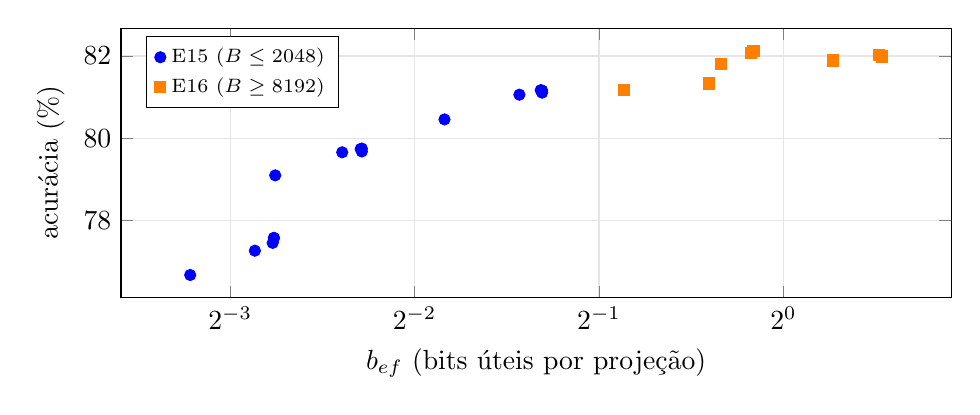
\begin{tikzpicture}
\begin{axis}[width=\columnwidth, height=5cm, xmode=log, log basis x=2, xlabel={$b_{\text{ef}}$ (bits úteis por projeção)}, ylabel={acurácia (\%)}, grid=major, grid style={gray!20}, legend style={font=\scriptsize, at={(0.03,0.97)}, anchor=north west}]
\addplot[only marks, blue, mark=*] coordinates {(0.1474,77.58) (0.1076,76.68) (0.1372,77.27) (0.1467,77.46) (0.1474,77.58) (0.2051,79.68) (0.1481,79.10) (0.1905,79.66) (0.2042,79.74) (0.2051,79.75) (0.4038,81.11) (0.2798,80.46) (0.3708,81.06) (0.4017,81.17) (0.4038,81.16)};
\addlegendentry{E15 ($B \le 2048$)}
\addplot[only marks, orange, mark=square*] coordinates {(0.8934,82.13) (0.5487,81.17) (0.7906,81.80) (0.8865,82.07) (1.4488,81.99) (0.7560,81.33) (1.2044,81.89) (1.4309,82.03)};
\addlegendentry{E16 ($B \ge 8192$)}
\end{axis}
\end{tikzpicture}
\caption{E15 e E16: acurácia contra a informação efetiva por projeção, nos canais ruidoso e float.}
\label{fig:e15}
\end{figure}}
\newcommand{\EdezesseisRdois}{0,83}
\newcommand{\EdezesseisRdoisNominal}{0,01}
\newcommand{\EdezesseisCelulas}{23}
\newcommand{\EquatorzeTabela}{%
\begin{table*}[t]
\centering
\caption{E14: acurácia de teste (\%) com projeções medidas por diferença central da perda, sem backpropagation (média de 2 sementes). \emph{abs}: cada perda lida por um conversor de $b$ bits em faixa fixa; \emph{difer}: a diferença lida diretamente, com faixa adaptada}
\label{tab:e14}
\begin{tabular}{rrccccccccc}
\toprule
$N$ & $r$ & exata & dif. & abs 8 & abs 12 & abs 16 & abs 20 & difer 1 & difer 2 & difer 4 \\
\midrule
13.002 & 8 & 69,6 & 69,5 & 27,7 & 56,4 & 69,6 & 69,5 & 61,6 & 70,4 & 69,6 \\
13.002 & 32 & 75,8 & 75,8 & 34,3 & 70,3 & 75,7 & 75,7 & 69,4 & 74,8 & 75,9 \\
13.002 & 128 & 78,8 & 78,9 & 48,5 & 75,8 & 78,8 & 78,8 & 73,7 & 78,1 & 78,7 \\
118.282 & 8 & 74,2 & 74,1 & 27,4 & 59,9 & 73,6 & 74,0 & 69,6 & 73,0 & 74,2 \\
118.282 & 32 & 77,6 & 77,6 & 34,0 & 69,7 & 77,4 & 77,5 & 73,1 & 76,5 & 77,5 \\
118.282 & 128 & 80,7 & 80,7 & 53,7 & 73,8 & 80,3 & 80,7 & 76,1 & 80,1 & 80,7 \\
\bottomrule
\end{tabular}
\end{table*}}
\newcommand{\EquatorzePum}{6}
\newcommand{\EquatorzePdois}{6}
\newcommand{\EquatorzePtres}{6}
\newcommand{\EquatorzePquatro}{6}
